\documentclass{article}
\usepackage{graphicx} % Required to insert images
\usepackage[hidelinks]{hyperref}

% Margins
\topmargin=-0.45in
\evensidemargin=0in
\oddsidemargin=0in
\textwidth=6.5in
\textheight=9.0in
\headsep=0.25in

\linespread{1.1} % Line spacing

\title{
\vspace{2in}
\textmd{\textbf{CPSC 471:\ Project Proposal}}\\
\normalsize\vspace{0.1in}\small{Due\ on\ February 3 \\ Group Number 3 \\ TA: Ibrahim Karakira}\\
\vspace{3in}
}

\author{Tanner Collin, Jordan Heinrichs, Ali Waseem}
\date{}

\begin{document}
\maketitle
\newpage

\section{Introduction}
The project will be an implementation of user driven rental service for cars.
Currently there are multiple car sharing companies on the market such as Car2Go \cite{car2go}
and Uber \cite{uber}, but there no easy to use service to rent your car out while you are not using it.
Our solution would create an easy to use and convenient way to do short term rentals on personal vehicles. The concept would be similar to Airbnb \cite{airbnb} but for vehicles.
We hope that we can make it easier for some people to make some money by loaning out their car and make it possible for people to save money on rentals.
The following proposal will cover the problem definition, solution, and our motivation for this product.

\section{Problem Definition}
\subsection{History of Problem}
For the longest time renting cars offered a small variety of choice for the user and expensive fixed rates.
It also didn't account for users that own cars and wanted people to rent them to make some income.
\subsection{Problem Intreset}
This problem allows us to create a service that can help car renters and car owners. By providing a peer-to-peer service,
users can have a much wider variety of vehicles to rent. This problem can also provide our group of total freedom on creating
this complex service that correlates to the material of CPSC 471.
\subsection{Occurance of Problem}
This problem can occur for multiple people for different reasons. For example: someone is going camping but needs a bigger car
than their sedan. With our service they can rent a bigger vehicle and submit their own vehicle up for rent.
\subsection{Current Solutions}
There are other solutions on the market for this service, but none of them exist in Calgary.
Our service can provide the people of Calgary a better and cheaper variety of cars to rent.
The major service that already exists is called GetAround \cite{getaround}, and it offers a lot of the same
features that we have purposed.
What makes our service distinct is the location we are offering, no other service like this exists in Calgary.

\section{Proposed Solution}
The end result of the project will create a product that will allow the user to have peer-to-peer ride sharing. It will be making use of a relational database for all persistent information.
The user will be able to log in and list his car at the set price or he could browse for all listed cars in a location.
All the transactions between users will also be done through the program.

The deliverables of this project will be a webapp with a user centric design with an easy to use interface. If time is permitted a mobile app will be created. Documentation on the RESTful API, user documentation on how to use the app, and the technical documentation on the database design will be delivered.

The feature set of the webapp and the mobile app will be identical.
The user will be able to login to their profile and access and edit their information such as phone number, address, bank information, and balance.
The user can list multiple cars that can be rented. Each car will have the model, type, year, location, and license plate. They can specify the price and the times that are available for renting.
The user can rent cars as well, they can search for cars by type, model, price, and year for renting. After the user find which car they wish to rent they may book it.
Bookings times are kept track, the user may edit or cancel the appointment as needed.
After the vehicle is rented, the balances of the renter and owner are updated.
The above user interactions will be made touch friendly and simple to use.

\section{Motivation}
Our solution is needed because people need transportation when they visit a new
city for business or vacation. In 2015, the car rental business was a 27
billion dollar industry \cite{marketdata}. We want to take some of that money
and help to put it back into the people's hands by allowing them to rent their
cars out.

Our project is unique in Calgary because no other service like this exists in
this city. Uber is similar to our solution, but is different because they are a
ride-sharing company and we are a car rental company. The users of our service
drive themselves.

Our project helps contribute to the economy by giving people another way to
make money and make use of vehicles that could otherwise be collecting dust. It
liberates people with another available mode of transportation and puts money
back in the public's hands.

\section{Conclusion}
Overall our project aims to create a service that provides peer-to-peer car rentals for the people of Calgary.
The application will be a RESTful server interacting with a web application and (if time permits) a mobile app.
We hope to change the way people rent cars within the city of Calgary

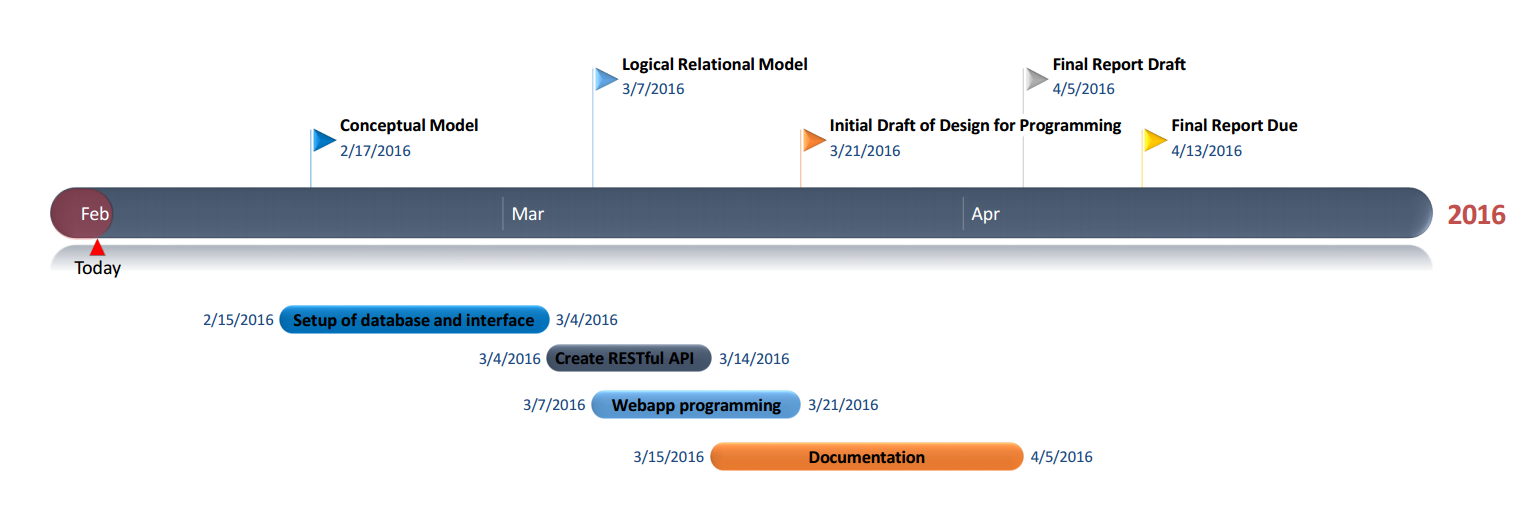
\includegraphics[scale=0.45,keepaspectratio]{Timeline}
\begin{thebibliography}{9}

\bibitem{getaround}
  GetAround,
  \url{https://www.getaround.com/}

\bibitem{car2go}
  Car2Go,
  \url{www.car2go.com}

\bibitem{uber}
  Uber,
  \url{www.uber.com}

\bibitem{airbnb}
  Airbnb,
  \url{www.airbnb.ca}

\bibitem{marketdata}
  AutoRental News,
  \url{http://www.autorentalnews.com/content/research-statistics.aspx}

\end{thebibliography}

\end{document}
